\chapter{Methods and Prototype}

In this section, the used methods are laid out and the implemented prototype is described. 
\section{Methods used}
\subsection{MapReduce}
At the very core of this thesis lies the idea of MapReduce, a programming model made popular by Google and presented in \cite{Dean2008}. Having large data sets to analyse that may not be handled by only few computers, like the millions of Websites gathered by Google each day that have to be indexed fast and reliably, MapReduce  provides a way of automatic parallelisation and distribution of large-scale computations. Users only need to define two types of functions: a map and a reduce function. Each computation expressed by these functions takes a set of input key/value pairs and produces a set of output key/value pairs.
A map function takes an input pair and produces a set of \textit{intermediate} key/value pairs. Once the intermediate values for each intermediate key \textit{I} are grouped together, they are passed to the reduce function. 
The reduce function then takes an intermediate key \textit{I} and the corresponding set of intermediate values (usually supplied as an iterator to the reduce function) and merges them according to user-specified code into a possibly smaller set of values. The resulting key and value are then written to an output file, allowing to handle lists of values that are too large to fit in memory. 

A very simple yet often used MapReduce operation is to count words in a collection of documents, the so called \textit{WordCount}. Below pseudocode demonstrates how one can count all the words in documents using map and reduce functions.

\begin{algorithmic}
\Function{map}{String key, String value}
\State \textit{// key: document name, value: document content}

\For{word $w$ in values}
\State EmitIntermediate($w$, $"1"$);
\EndFor
\EndFunction


\Function{reduce}{String key, Iterator values}
\State \textit{// key: a word, values: a list of "1"'s}
\State int $result$ = 0;
\For{$v$ in values}
\State $result$ += ParseInt($v$);
\EndFor
\State Emit(AsString($result$));
\EndFunction
\end{algorithmic}

The map function splits the received text (\textit{value}) into all corresponding words and for each word, emits its occurrence count (simply a 1). The reduce function then takes, for each word (\textit{key} of the reduce function) individually, these occurrences (\textit{values}) and sums them up, eventually emitting for each word the sum of occurrences (\textit{result}). Although above pseudocode suggests inputs and outputs to be strings, the user specifies the associated types. This means that input keys and values may be of a different domain than the output keys and values (note that the \textit{intermediate} keys and values are from the same domain as the output keys and values). Conceptually, this is expressed as follows:
\newline
\newline
\begin{tabular}{lll}
map	& (k1, v1) & $\to$ list(k2, v2)\\
reduce & (k2, list(v2)) & $\to$ list(v2)
\end{tabular}

The traditional way to view the workflow in a MapReduce program is indicated by Figure \ref{fig:mapreduce_workflow}. A master schedules execution and assigns tasks to workers, which then perform the actual map or reduce on the assigned data. Input data is partitioned into \textit{M} splits with a size of around 16-64 MB per piece to be processed in parallel by different machines, and the intermediate key space is partitioned into \textit{R} pieces, where R usually is the number of available workers for executing reduce but may also be specified by the user. To evenly distribute these pieces, a partitioning function like \textit{hash(key) mod R} may be used. In such a setting, same intermediate keys may not be grouped together, which is done before the reduce action is performed. Additional combination in between may be applied to reduce the amount of data to be distributed among the workers.

\begin{figure}
	\centering	
	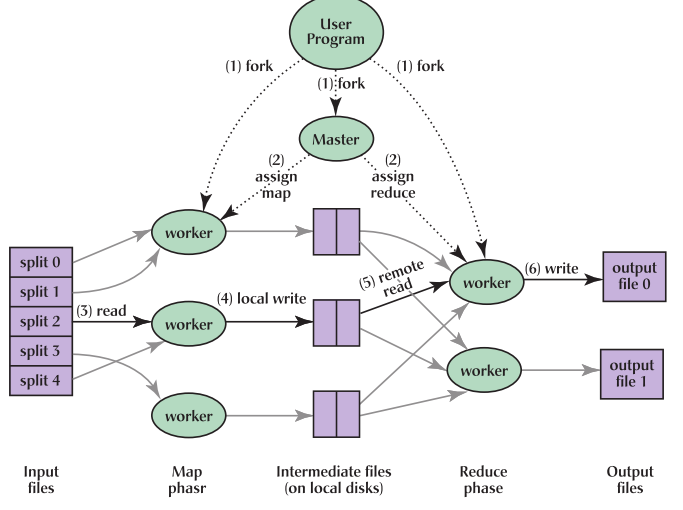
\includegraphics{mapreduce_workflow}
	\caption{Execution overview in a typical MapReduce program}	
	\label{fig:mapreduce_workflow}
\end{figure} 
\section{Peer-to-Peer Overlay Networks}
\subsection{Definitions and Flavours}
Peer-to-peer (P2P) systems and applications are distributed systems without any centralized control or hierarchical organisation, where the software running at each node is equivalent in functionality \cite{Stoica2001}. Instead of a central server (as present in Client/Server architectures \cite{Schollmeier:2001:DPN:882470.883282}), many hosts (usually referred to as peers) that posses desired contents also handle user requests for them \cite{Chawathe2003}. According to \cite{Schollmeier:2001:DPN:882470.883282}, a P2P network is given if the participants share a part of their own hardware resources (like e.g. processing power or storage capacity), which provide the service and content offered by the network and which are directly accessible by other peers. Peers are, thus, both resource (service  and content) providers and requesters. There exist different flavours of P2P overlay networks but the overall themes may be summarised as "pure" P2P and "hybrid" P2P systems. In a \textit{pure P2P system}, any entity may be removed without the network suffering any service loss. A \textit{hybrid P2P system}, on the other hand, requires a central entity to provide parts of the offered networks. An example of such a hybrid system was Napster\cite{Chawathe2003}.  
\subsection{Discovering Content and Distributed Hash Tables}
The definitions given above demonstrate the need for efficiently discovering content and/or services without using a central server. Central servers may provide O(\textit{1}) lookup of a file's location in the P2P network but also suffers from the problem of being a single point of failure (SPOF), which made Napster very efficient for lookup but also vulnerable for lawsuits\cite{Chawathe2003} and certainly not scalable at that time\cite{Ratnasamy:2001:SCN:964723.383072}. However, although being rather resilient to node crashes, without efficient lookup capabilities, P2P networks are \textit{unstructured} and as there is no constraint on where files are placed in the overlay network, queries need to be flooded across the overlay to find the location of the desired content (requiring O(\textit{n}) lookups). Such overlay networks like e.g. Gnutella were, therefore, not scaling. To overcome this, distributed hash tables (DHTs) were introduced, of which the Content-Addressable Network (CAN, \cite{Ratnasamy:2001:SCN:964723.383072}) may be one of the first such design outlines intended to be used in P2P networks. Keys are mapped onto values in a DHT, operations include (among others) typical hash table or hash map operations like put(\textit{key}, \textit{value}), get(\textit{key}): \textit{value}, etc. The idea is that the problem of P2P systems is not the file transfer process which is inherently scalable but finding the peer from whom to retrieve the file\cite{Ratnasamy:2001:SCN:964723.383072}. Thus the indexing scheme needs to be scalable to make the whole P2P system scalable. Importantly, it requires no centralized control and there is no rigid hierarchical naming structure like e.g. in IP or DNS routing. DHTs make overlay networks \textit{structured} and provide hash-table-like semantics on internet-like scales \cite{Ratnasamy:2001:SCN:964723.383072}. Efficient routing protocols (e.g. Chord\cite{Stoica2001}, Kademlia\cite{Maymounkov:2002:KPI:646334.687801}) reduce lookup complexity to O(log \textit{n}) while lowering node state (the routing entries to other nodes) to O(log \textit{n}) as well. Although there are some limitations to DHTs (e.g. a high churn rate requires O(log \textit{n}) repair operations, keyword searches DHTs by default may only handle exact-match lookups, and many queries may not require an exact recall as they are mostly for well-replicated files and thus, do not justify the overhead of a DHT\cite{Chawathe2003}), they provide a good balance between node state and communication overhead. As TomP2P uses Kademlia as its DHT, its functionality will be briefly outlined next. For more detailed information, please consult the accompanied references.
\subsubsection{Kademlia}
Kademlia is a P2P DHT with XOR-based metric topology \cite{Maymounkov:2002:KPI:646334.687801}. It combines provable consistency and performance, latency-minimising routing, and a symmetric, unidirectional topology. It minimises number of configuration messages nodes must send to learn about each other, and configuration information spreads automatically as a side-effect of key lookups. Furthermore, nodes have enough knowledge and flexibility to route queries through low-latency paths.
Kademlia contacts only O(log \textit{n}) nodes while searching the system containing \textit{n} nodes. Keys are 160-bit opaque quantities of which each participating computer is assigned one node ID in the 160-bit key space. Key-value pairs are stored on nodes with IDs "close" to the key. Closeness is defined as the bitwise exclusive or (XOR) distance of two nodes' IDs (d(x, y) = x $\mathbin{\oplus}$ y, where x and y are two 160-bit identifiers). A node's ID is a large random number intended to achieve uniqueness. Thus, distance is not used in a geographical sense as "neighbour" nodes may be spread around the world and are only logically considered close in the overlay network due to their small XOR distance. Kademlia treats nodes as leaves in a binary tree, with each node's position determined by the shortest unique prefix of its ID. In a fully-populated binary tree of 160-bit IDs, the magnitude of the distance between two IDs is the hight of the smallest subtree containing them both. If the binary tree is not fully populated, the closest leaf to an ID is the leaf whose ID shares the longest common prefix. For every node, the binary tree is divided into a series of successively lower subtrees that do not contain the node. Every node knows at least one node in each of its subtrees if the subtree contains a node. By successfully querying the known node, contacts are found in lower subtrees until the lookup finally converges to the target node.Thus, any node can locate any other node by its ID.
A Kademlia node stores contact information about each other to route query messages for nodes of distance $2^i$ and $2^{i+1}$ (called \textit{k}-buckets). \textit{k}-buckets are sorted by time last seen (least-recently (head) to most-recently (tail) Appropriate \textit{k}-buckets are updated whenever a Kademlia node receives any message (request or reply) from another node. 


\section{Prototype}
